\documentclass[12pt]{article}

\usepackage[utf8]{inputenc}
\usepackage{geometry}
\geometry{a4paper,scale=0.75}
\linespread{1.5}
\usepackage{graphicx} 
\usepackage{float} 
\usepackage{subfig} 
\usepackage{enumerate}
\usepackage{enumitem}
\usepackage{amsmath}
\usepackage{array}
\usepackage{booktabs}
\usepackage{multirow}
\usepackage{amsfonts}
\usepackage[english]{babel}
\usepackage{amsthm}
\usepackage{dcolumn}
\usepackage{multicol}
\usepackage{stfloats}
\usepackage{lscape}
\usepackage[figuresright]{rotating}
\RequirePackage{pdflscape}
\usepackage[toc,page]{appendix}
\usepackage{geometry}
\usepackage{longtable}
\usepackage{comment}
\usepackage{xcolor}

% -------- enumerated sub-labels (a), (b), … --
\usepackage{enumitem}
\setlist[enumerate,1]{label=(\alph*),ref=\alph*}
% ---------------------------------------------

\usepackage{hyperref}
\hypersetup{hidelinks,
	colorlinks=true,
	allcolors=black,
	pdfstartview=Fit,
	breaklinks=true}
\usepackage{csquotes}
\usepackage{natbib}
\bibliographystyle{apalike}
\newtheorem{definition}{Definition}
\newtheorem{theorem}{Theorem}
\newtheorem{proposition}[theorem]{Proposition}
\newtheorem{lemma}[theorem]{Lemma}
\newtheorem{corollary}[theorem]{Corollary}
\newtheorem*{remark}{Remark}
\newtheorem{example}{Example}
\newtheorem{exercise}{Exercise}
\newtheorem{assumption}{Assumption}[section] % number within sections


\begin{document}

\begin{center}
    ECON 3123: Macroeconomic Theory I\\
    {\large \textbf{Tutorial Note 4: IS-LM Framework}}\\
    Teaching Assistant: Harlly Zhou
\end{center}

\subsection*{Basic IS-LM Model}
\paragraph{Deriving the Model}
Recall that in the goods market, the deamnd for goods is
\[ Z = C + I + G. \]
Recall that consumption depends on disposable income $Y-T$. And in reality, investment depends on output and interest rate:
\[ I = I (Y,i),\]
where $I$ increases with $Y$ and decreases with $i$. (Think about the intuition.)

Then we rewrite the demand as
\[ Z = C(Y-T) + I(Y,i) + G.\]
At equilibrium, we have
\[ Y = Z.\]
This determines the equilibrium output $Y^*$. When the nominal interest rate increases, the investment will decrease, shifting the $ZZ$ curve downwards. We have the new equilibrium output $Y'$, shown as Figure \ref{fig:is_01}.

\begin{figure}[htp]
    \centering
    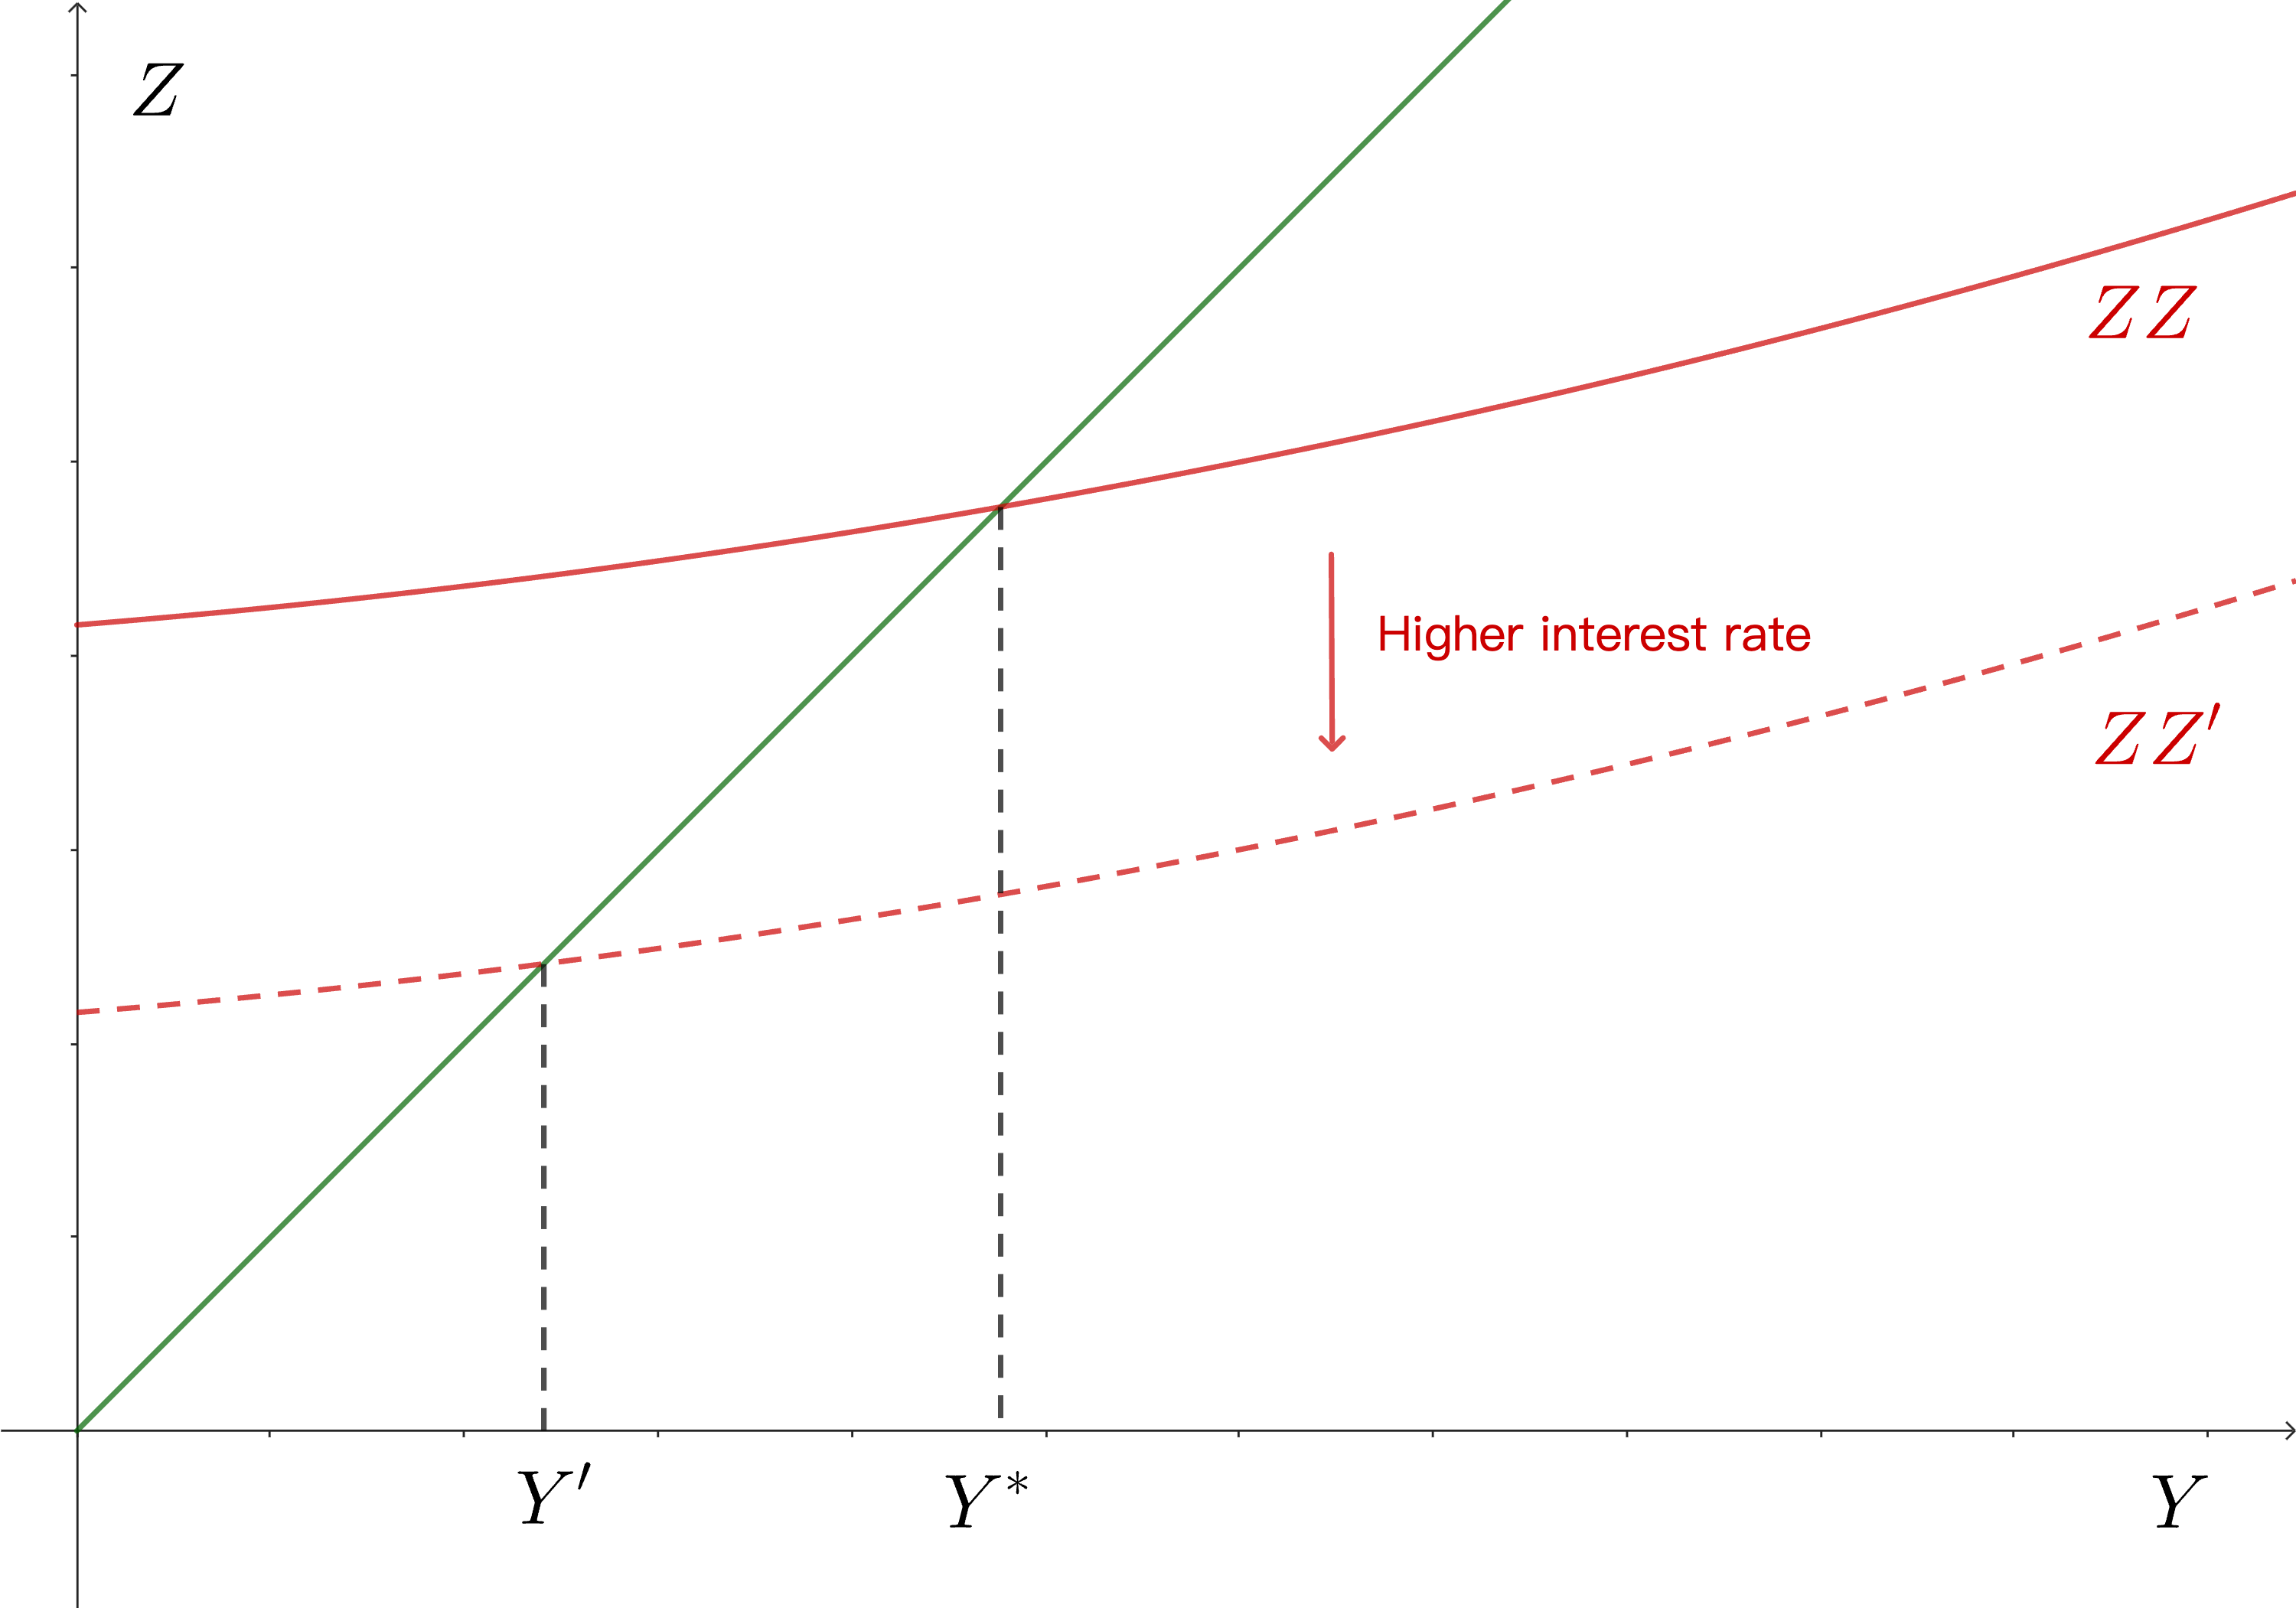
\includegraphics[width=0.6\textwidth]{is_01.png}
    \caption{Goods Market Equilibrium}
    \label{fig:is_01}
\end{figure}

If we put the interest rate and the output together, then we get the IS relation (Figrue \ref{fig:is_02}).\

\begin{figure}[htp]
    \centering
    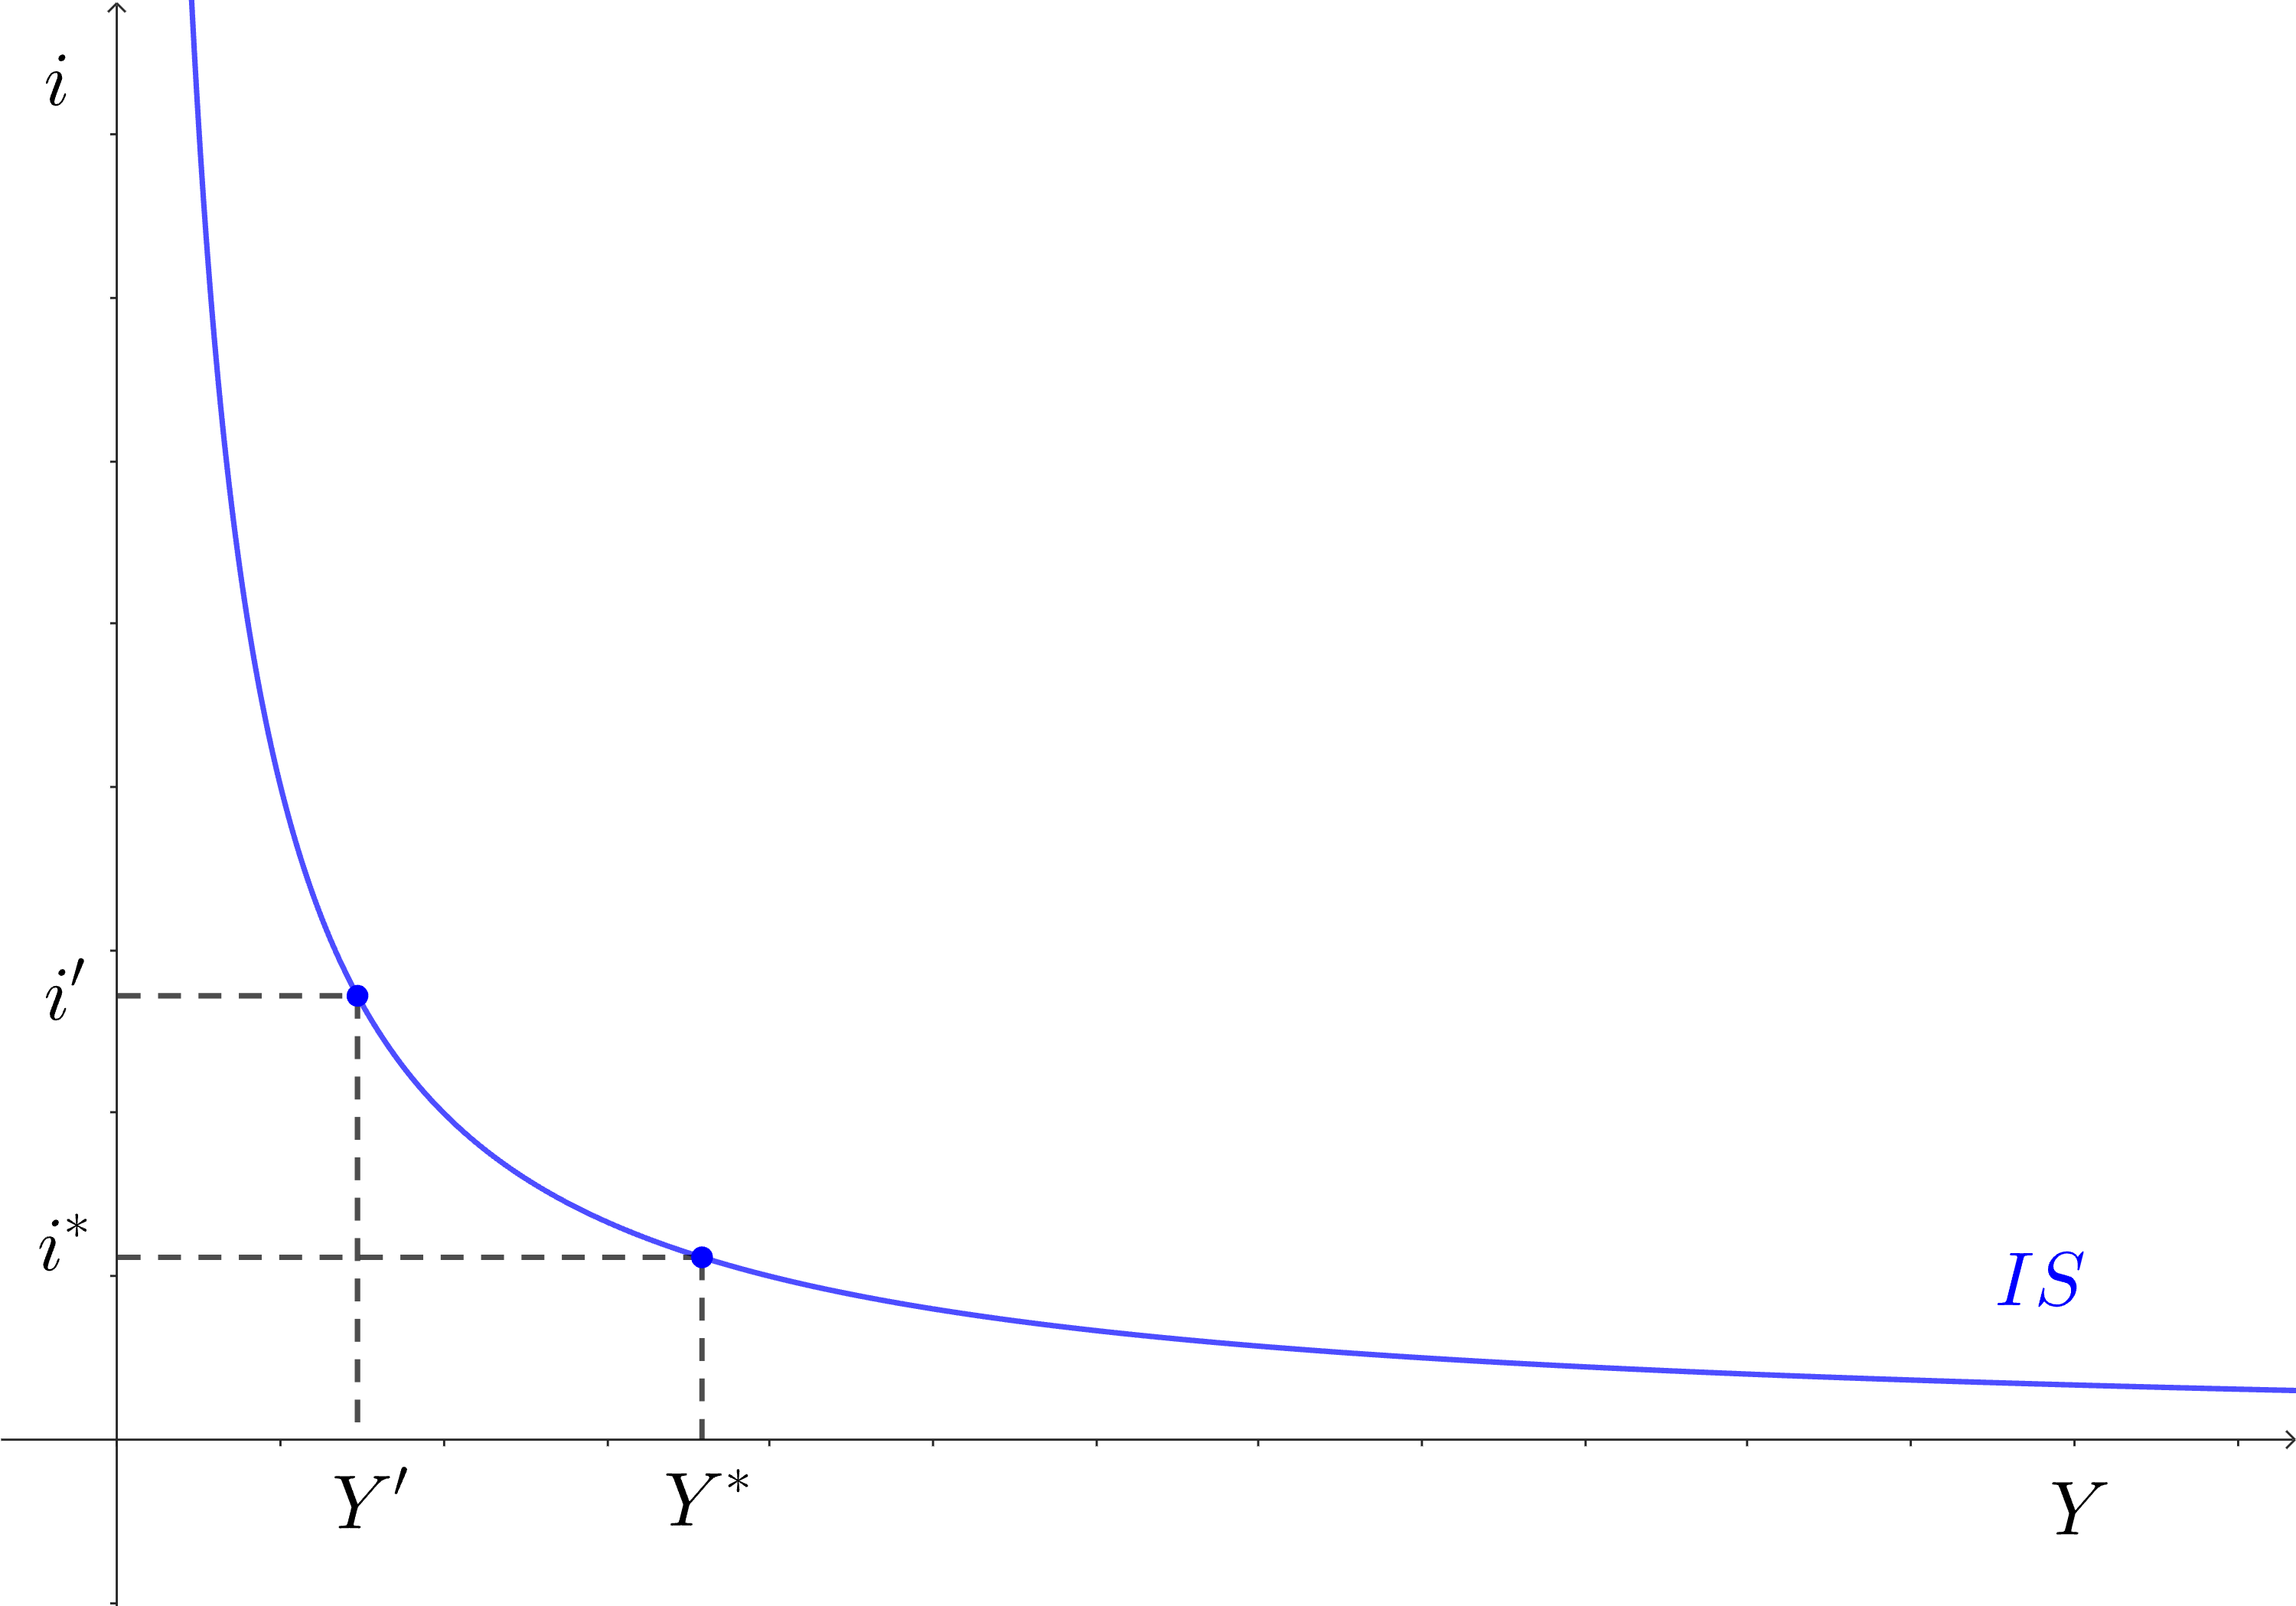
\includegraphics[width=0.6\textwidth]{is_02.png}
    \caption{Deriving IS curve from goods market equilibrium}
    \label{fig:is_02}
\end{figure}

Note that all the pairs $(i, Y)$ is a pair of \textbf{equilibrium} values of nominal interest and output.

In the derivation of the IS relation, note that the output is measured in \textit{real temr}. Therefore, we should also use real term in the money market equilibrium to derive the \textbf{LM relation}. Recall that the nominal money demand is
\[M^d = \$ Y L(i)\]
for some decreasing function $L(i)$. The real money demand is
\[\frac{M^d}{P} = Y L(i).\]
At equilibrium, $M^d = M^S = M$. In the short run, we assume that prices are sticky. Hence, we have
\[ \frac{M}{P} = Y L(i).\]
Central banks adjust money supply $M$ to target an interest rate $i = \bar{i}$. Hence, the LM curve is a horizontal line. Putting together with the IS curve, we get Figure \ref{fig:is-lm}.

\begin{figure}[htp]
    \centering
    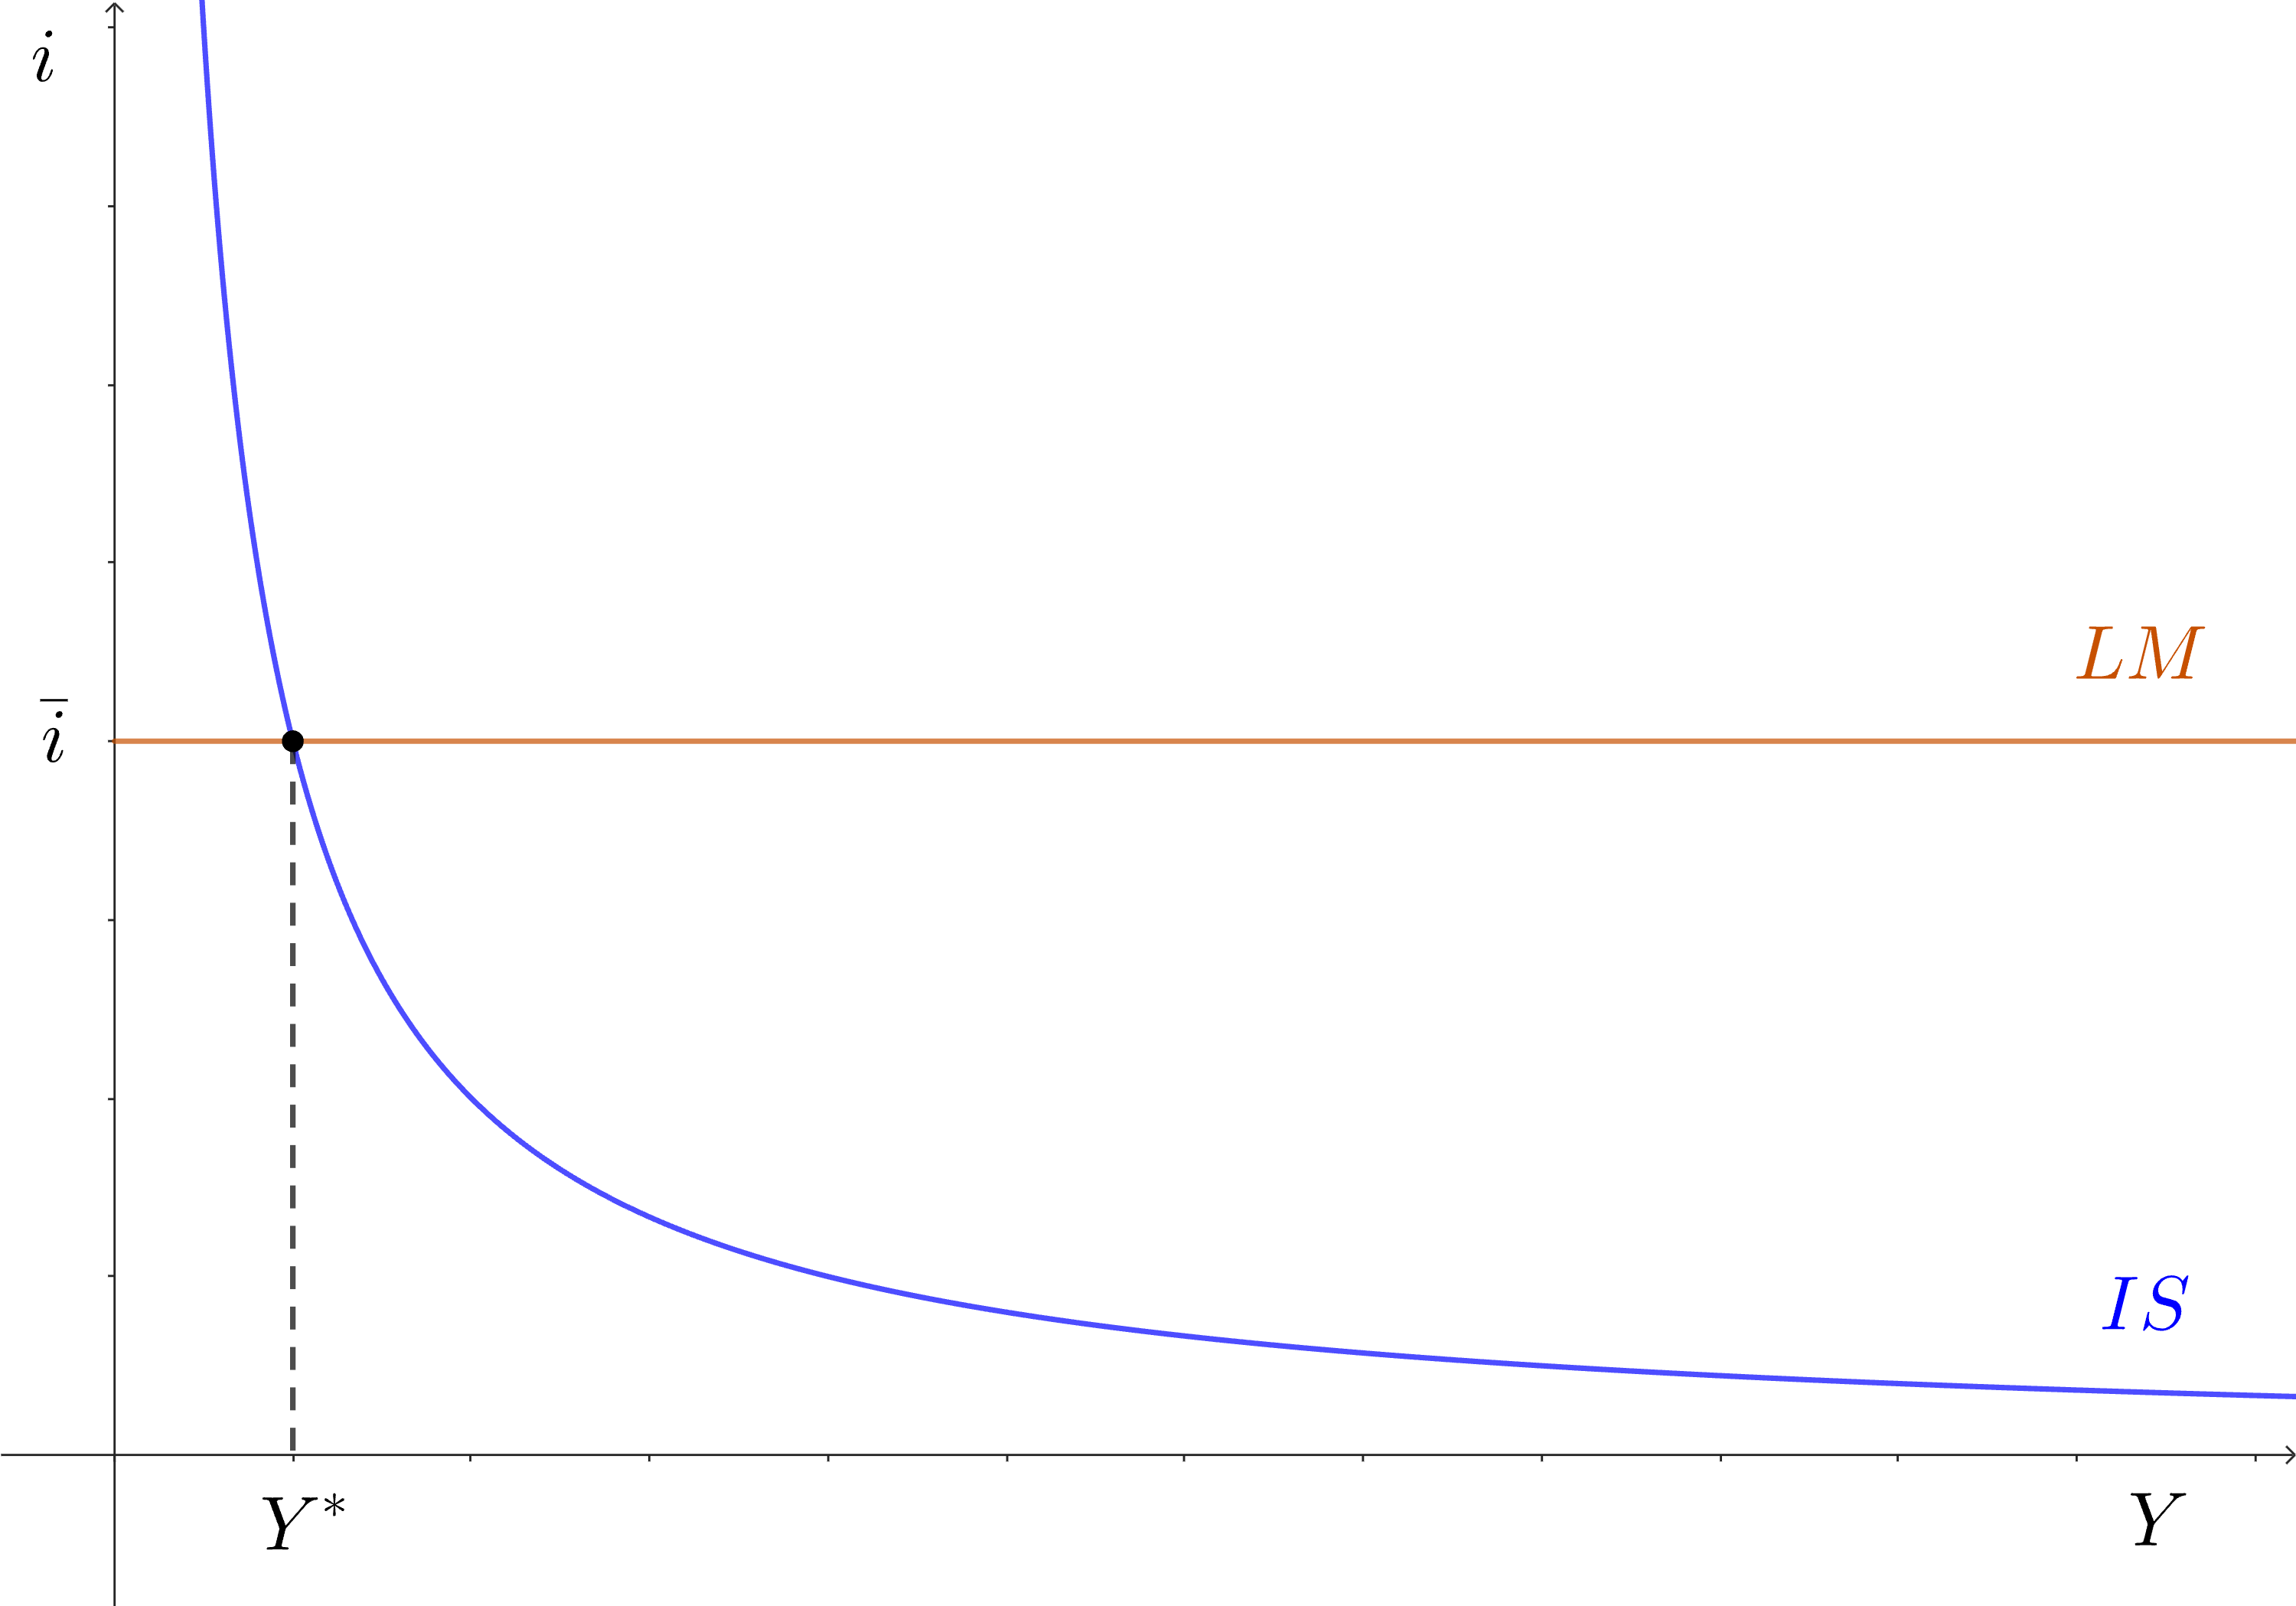
\includegraphics[width=0.6\textwidth]{is-lm.png}
    \caption{IS-LM Framework}
    \label{fig:is-lm}
\end{figure}

They together yield the \textbf{general equilibrium} interest rate and output, $(\bar{i}, Y^*)$.

\begin{exercise}
    Chapter 5, Question 5 in Blanchard, Olivier (2021), \textit{Macroeconomics}, 8th ed., Pearson.
\end{exercise}

\begin{exercise}
    \begin{enumerate}[label=(\arabic*)]
        \item At a given interest rate level, a temporary reduction in government purchases will
        \begin{enumerate}[label=\Alph*.]
            \item increase desired saving, causing the IS curve to shift down and to the left.
            \item increase desired saving, causing the IS curve to shift up and to the right.
            \item decrease desired saving, causing the IS curve to shift down and to the left.
            \item decrease desired saving, causing the IS curve to shift up and to the right.
        \end{enumerate}
        \item When all markets in the economy are simultaneously in equilibrium, we say
        \begin{enumerate}[label=\Alph*.]
            \item markets are complete.
            \item markets are perfect.
            \item there is disequilibrium.
            \item there is general equilibrium.
        \end{enumerate}
        \item If government spending and taxes increase by the same amount, the IS curve will
        \begin{enumerate}[label=\Alph*.]
            \item shift to the left.
            \item shift to the right.
            \item stay unchanged.
            \item have an ambiguous shift.
        \end{enumerate}
    \end{enumerate}
\end{exercise}

\subsection*{Introducing Financial Sector}
\paragraph{The Fisher Equation}
By no-arbitrage condition, we have
\[ 1 + r_t = \frac{(1 + i_t) P_t}{P^e_{t+1}}.\]
Since
\[\pi^e_{t+1} = \frac{P^e_{t+1}-P_t}{P_t},\]
we obtain
\[1 + r_t = \frac{1 + i_t}{1 + \pi^e_{t+1}}.\]
By an approximation, we obtain the \textbf{Fisher Equation}:
\[r_t \approx i_t = \pi^e_{t+1}.\]

\begin{example}[No-arbitrage condition]
    Consider a one-year risk-free bond with face value \$1,000. Suppose the risk-free interest rate is 5\%. The bond is sold at \$980 today.
    \begin{enumerate}[label=(\arabic*)]
        \item Is there any arbitrage opportunity? Describe how to make a profit. Assume that you are allowed to lend and borrow at the risk-free interest rate.
        \item To avoid arbitrage, the issuer would like to provide some coupon. Coupon is some reward to the investors in addition to the interests which is distributed at the end of each period (annually, semi-annually, etc., depending on the specified rule. Assume that coupon is distributed annually here). Then what should be the coupon rate, i.e., the ratio of the amount of coupon to the face value?
    \end{enumerate}
\end{example}


\paragraph{Risk Premium}
To hedge the default risk, the bank always charge a risk premium $x$ other than the real rate for firm financing. Therefore, instead of having $I = I(Y,i)$, we have
\[ I = I (Y, r+x) = I(Y, i-\pi^e+x).\]

\begin{example}[No-arbitrage condition]
    Consider a zero-coupon one-year bond with face value \$1,000. The risk-free interest rate is 5\%. However, there is default risk on this bond. It has probability of 20\% to pay only \$800 back to the investor and 80\% probability to pay \$1,000 back. 
    \begin{enumerate}[label=(\arabic*)]
        \item If the risky bond has its bond rate equal to the risk-free rate, then what should be the bond price?
        \item If the risky bond has the same price as the risk-free bond today, what will be the risk premium?
    \end{enumerate}
\end{example}

\paragraph{Solvency, Liquidity, and Bank Runs}
\textbf{Solvency} measures a financial intermediary's ability to pay its liabilities. At a simplified level, you can just compare the cash it owns and the liabilities it owes. \textbf{Liquidity} measures how easy an asset can be transformed into cash. They are related in the following sense:
\begin{itemize}
    \item If the assets are illiquid, \textit{i.e.,} hard to be transformed into cash, then the financial intermediary is likely to be more insolvent and to have more risk of going bankrupt.
    \item If the liabilities are liquid, \textit{i.e.,} easy to be asked to pay in cash, then the financial intermediary is likely to be more insolvent and to have more risk of going bankrupt.
\end{itemize}

\begin{exercise}
    Chapter 6, Question 4 in Blanchard, Olivier (2021), \textit{Macroeconomics}, 8th ed., Pearson.
\end{exercise}

\subsection*{Extended IS-LM Framework}
To understand financial shocks using the IS-LM framework, we need two main modifications:
\begin{itemize}
    \item Distinguish nominal interest rate from the real interest rate;
    \item Incorporate risks into the model.
\end{itemize}
Then we have the following IS relation and LM relation:
\begin{align*}
    \text{IS relation}: &\, Y = C(Y-T) + I(Y, r+x) + G\\
    \text{LM relation}: &\, r = \bar{r}.
\end{align*}
By the Fisher equation, there is a lower bound for the real interest rate: $r \geq -\pi^e$.

\begin{example}
    Consider the following behavioral equations:
    \begin{align*}
        C &= 200 + 0.5(Y-T)\\
        I &= 500 - 2000(r+x) + 0.3Y
    \end{align*}
    and the real money demand:
    \begin{align*}
        \frac{M^d}{P} = Y(0.8-5\bar{i}).
    \end{align*}
    Suppose that $G = 100$ and $T = 200$. The price level is 10, and the nominal money supply is 13000. The expected inflation is $2\%$, and the risk premium is $5\%$.
    \begin{enumerate}[label=(\arabic*)]
        \item Solve for the equilibrium output. What is the target nominal interest rate?
        \item Can the central bank expand the money supply to 21,000? What nominal interest rate is it targeting?
        \item What is the lower bound for real interest rate target? What is the upper bound for nominal money supply?
        \item Keep the target rate as in part (1). Find the upper bound of tax such that there exists a positive equilibrium output.
        \item Suppose that people become pessimistic on the economy, and become more risk averse on assets. What is the effect of this? Illustrate this economy in a diagram. Explain your figure in words.
    \end{enumerate}
\end{example}

\subsection*{Policy Analyses Exercises}
\begin{example}\label{eg:arg}
    Consider an economy like Argentina in 2001. Due to rampant corruption from the government, massive tax evasion, and money laundering activities, both consumers and investors become very pessimistic about the Argentine economy. Suppose initially, the economy is in an equilibrium. 
    \begin{enumerate}[label=(\arabic*)]
        \item Explain what happens to the economy in the short run when people become pessimistic about the economy. What will happen to output and the real interest rate?
        \item If you are the government of Argentina, what would you do with government spending in order to offset the effects of the pessimism? What will happen to output, the real interest rate, investment, and the consumption as the result of the government's action?
        \item If you are the central bank of Argentina, what kind of monetary policy that you can implement in order to offset the effects of the pessimism? What will happen to output, the real interest rate, investment, and the consumption as the result of the central bank's action?
    \end{enumerate}
\end{example}

\begin{exercise}
    Continue with Example \ref{eg:arg}. Suppose the Argentine government has very limited fiscal space, and it is already running very high budget deficit so that the government is very likely to default on its debt, and simultaneously, the nominal interest rate in Argentina is very close to zero, or the zero lower bound (ZLB). 
    \begin{enumerate}[label=(\arabic*)]
        \item Is it still appropriate to use the policy suggested in part (2)? Why?
        \item Is it still appropriate to use the policy suggested in part (3)? Why?
        \item What kind of policies can be implemented in order to offset the effects of the pessimism? Please suggest at least 1 policy and explain why it works.
    \end{enumerate}
\end{exercise}

\begin{exercise}
    Chapter 6, Question 9 in Blanchard, Olivier (2021), \textit{Macroeconomics}, 8th ed., Pearson.
\end{exercise}
\end{document}